\section{Section ???}

\subsection{Fractions {\tt <mfrac>}}

The {\tt mfrac} element is used for fractions. It can also be used to mark up
fraction-like objects such as binomial coefficients and Legendre symbols.
The syntax for {\tt mfrac} is

\begin{lstlisting}
  <mfrac> numerator denominator </mfrac>
\end{lstlisting}

The {\tt mfrac} element sets {\tt displaystyle} to "false", or if it was
already false increments scriptlevel by 1, within numerator and denominator.
This can be achieved with the following style in the user agent stylesheet:

\begin{lstlisting}
  mfrac > * {
    mathml-script-level: auto;
    mathml-math-style: inline;
  }
\end{lstlisting}

The default line thickness is given by FractionRuleThickness
Use the {\tt linethickness} attribute \cite{MathML3} to determine the
actual thickness of the fraction bar. A percent or unitless length is
interpreted as a multiple of the default rule thickness and
the named values "thin", "medium" and "thick" are interpreted as
50\%, 100\%, 200\%.

If the actual linethickness is nonzero, the {\tt mfrac} element is layout as
shown on \ref{FractionBoxModel}. The width is given by the maximum width of the
numerator and denominator and the numerator and denominator are horizontally
centered. A fraction bar with the actual thickness is drawn centered on the
axis height. The numerator and denominator are shifted
up and down using the values {\tt FractionNumeratorShiftUp},
{\tt FractionDenominatorShiftDown} in inline style and
{\tt FractionNumeratorDisplayStyleShiftUp},
{\tt FractionDenominatorDisplayStyleShiftDown} in display style.
If necessary, these shift values are increased to ensure that the gaps between
the numerator/denominator and fraction bar satisfy the minimal values provided
by {\tt FractionDenominatorGapMin} and
{\tt FractionNumeratorGapMin} in inline style and
{\tt FractionDenominatorDisplayStyleGapMin} and
{\tt FractionNumeratorDisplayStyleGapMin} in display style.

\begin{figure}
\centering
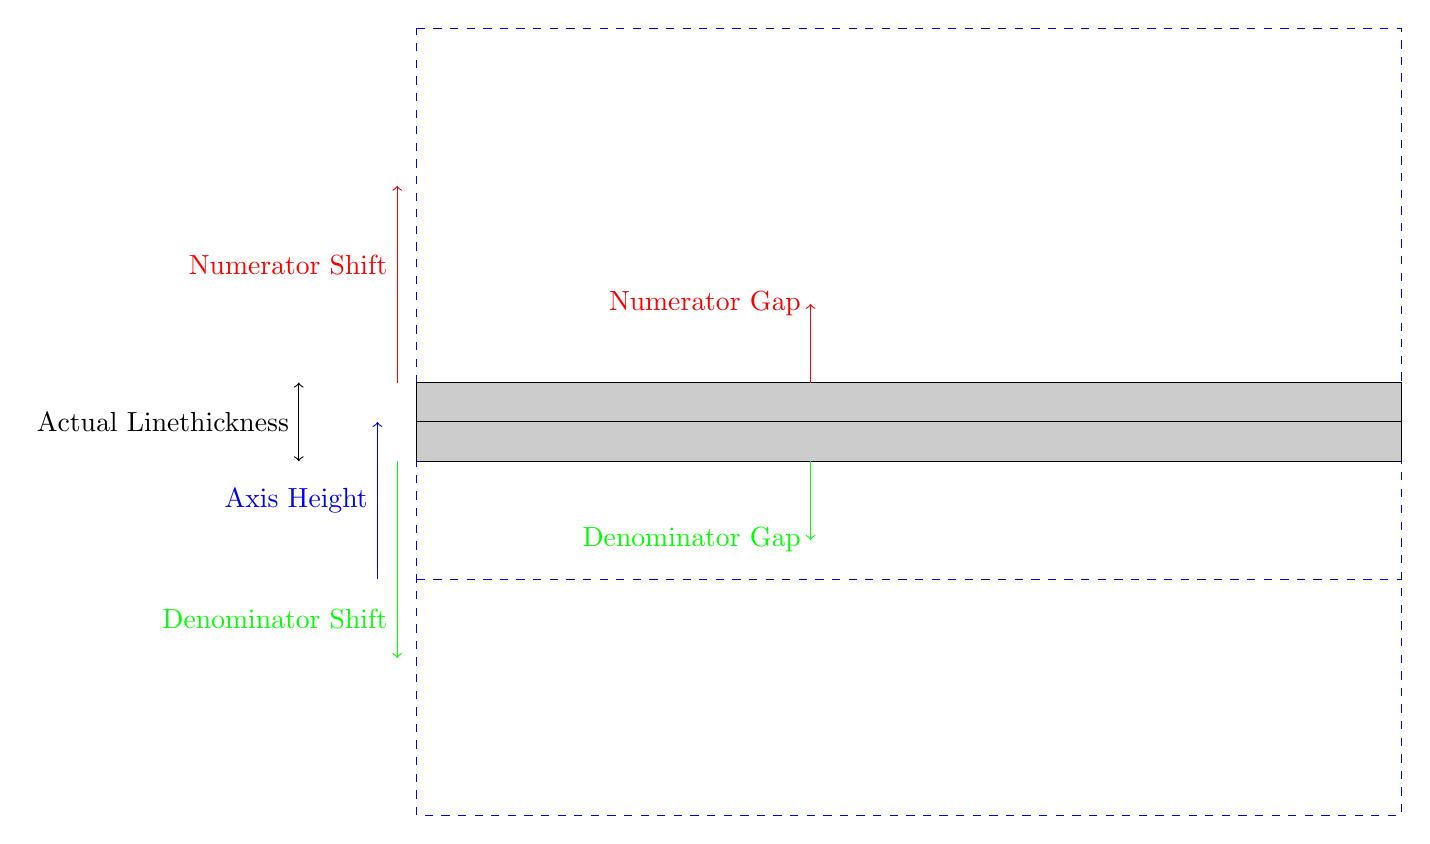
\begin{tikzpicture}[yscale=-1]
  \MathMLBox{0}{-5}{2.5}{1}{red}
  \MathMLBox{3.75}{1}{1}{1}{green}
  \draw[dashed,blue] (0,-7) -- (12.5,-7) -- (12.5,3) -- (0,3) -- cycle
  (0,0) -- (12.5,0);
  \fill[black!20] (0,-2.5) -- (12.5,-2.5) -- (12.5,-1.5) -- (0,-1.5) -- cycle;
  \draw[black] (0,-2.5) -- (12.5,-2.5) -- (12.5,-1.5) -- (0,-1.5) -- cycle
  (0,-2) -- (12.5,-2);
  \draw[->,blue] (-.5,0) -- (-.5,-1) node[left]{Axis Height} -- (-.5,-2);
  \draw[<->,black] (-1.5,-2.5) --
  (-1.5,-2) node[left]{Actual Linethickness} -- (-1.5,-1.5);
  \draw[->,red] (-.25,-2.5) -- (-.25,-4)
  node[left]{Numerator Shift} -- (-.25,-5);
  \draw[->,green] (-.25,-1.5) -- (-.25,.5)
  node[left]{Denominator Shift} -- (-.25,1);
  \draw[->,red] (5,-2.5) -- (5,-3.5) node[left]{Numerator Gap};
  \draw[->,green] (5,-1.5) -- (5,-.5) node[left]{Denominator Gap};
\end{tikzpicture}
\label{FractionBoxModel}
\end{figure}

If the actual linethickness zero, the {\tt mfrac} element is instead layout as
shown on \ref{StackBoxModel}. The relevant shift values are now
{\tt StackTopShiftUp},
{\tt StackBottomShiftDown} in inline style and
{\tt StackTopDisplayStyleShiftUp},
{\tt StackBottomDisplayStyleShiftDown} in display style.
If necessary, the two shift values are increased by a same value to ensure
the gaps between the top and bottom boxes satisfy the values provided by
by {\tt StackGapMin} in inline style and
{\tt StackDisplayStyleGapMin} in display style.

\begin{figure}
\centering
\begin{tikzpicture}[yscale=-1]
  \MathMLBox{0}{-5}{2.5}{1}{red}
  \MathMLBox{3.75}{1}{1}{1}{green}
  \draw[dashed,blue] (0,-7) -- (12.5,-7) -- (12.5,3) -- (0,3) -- cycle
  (0,0) -- (12.5,0);
  \draw[black,dashed] (0,-2) -- (12.5,-2);
  \draw[->,blue] (-.5,0) -- (-.5,-1) node[left]{Axis Height} -- (-.5,-2);
  \draw[->,red] (-.25,-2) -- (-.25,-4)
  node[left]{Stack Top Shift} -- (-.25,-5);
  \draw[->,green] (-.25,-2) -- (-.25,.5)
  node[left]{Stack Bottom Shift} -- (-.25,1);
  \draw[<->,blue] (5,-3.5) -- (5,-1.5) node[left]{Stack Gap} --
  (5,-.5);
\end{tikzpicture}
\label{StackBoxModel}
\end{figure}


User agents may increase the width by adding a trailing/leading space
of 1 pixel around the fraction. If the numerator is an embellished operator and
the {\tt mfrac} element is the outermost element in this embellished operator
hierarchy then the operator leading and trailing spaces must be added around
the fraction.

User agents may extend the box model to support the {\tt numalign},
{\tt denomalign} and {\tt bevelled} attributes \cite{MathML3}.
